\begin{sol}{empty-probability}
    Let $A_n=\varnothing$ for all positive integers $n$ and denote. Then we can use the third axiom (condition) of probability on these sets as they are pairwise disjoint ($\varnothing\cap\varnothing=\varnothing$) to get
    \[
        \PP(\varnothing)=\PP\left(\bigcup_{i=1}^{\infty}A_i\right)=\sum_{i=1}^{\infty}\PP(A_i)=\sum_{i=1}^{\infty}\PP(\varnothing),
    \]
    therefore $\PP(\varnothing)=0$, because otherwise the sum $\sum_{i=1}^{\infty}\PP(\varnothing)$ would diverge to infinity.
\end{sol}

\begin{sol}{nonempty-sample-space}
    According to the previous exercise $\PP(\varnothing)=0$, which would contradict the second axiom of probability, namely $\PP(\Omega)=1$, if $\Omega=\varnothing$.
\end{sol}

\begin{sol}{coin1}
    We can use the sample space $\Omega=\{H,T\}^3=\{(H,H,H),(H,H,T),\ldots,(T,T,T)\}$, where each elementary outcome has probability $\frac18$. The probability of getting exactly two heads is the probability of the event $\{(H,H,T),(H,T,H),(T,H,H)\}$, which is $\frac38$.
\end{sol}

\begin{sol}{twodie1}
    One way of modeling this experiment is to use the probability space $(\Omega,\mathcal{F},\PP)$, where $\Omega=\{1,2,\ldots,6\}^2=\{(1,1),(1,2),\ldots,(6,6)\}$, $\mathcal{F}=2^\Omega$, and $\PP(A)=\frac{|A|}{|\Omega|}=\frac{|A|}{36}$ for $A\in\mathcal{F}$. Let $B$ be the event of the sum being $7$. Then $B=\{(1,6),(2,5),(3,4),(4,3),(5,2),(6,1)\}$, and therefore $\PP(B)=\frac{|B|}{36}=\frac{6}{36}=\frac{1}{6}$.
\end{sol}

\begin{sol}{monotonicity}
    Set $A_1=A$, $A_2=B\setminus A$, and $A_i=\varnothing$ for all integers $i\ge3$. Then the events $A_i$ are pairwise disjoint and $\bigcup_{i=1}^{\infty}A_i=A\cup(B\setminus A)=B$, so it follows from the third axiom of probability that
    \[
        \PP(B)=\PP\left(\bigcup_{i=1}^{\infty}A_i\right)=\sum_{i=1}^{\infty}\PP(A_i)=\PP(A)+\PP(B\setminus A)+0+0+\cdots=\PP(A)+\PP(B\setminus A),
    \]
    which means that $\PP(B)\ge\PP(A)$ because $\PP(B\setminus A)\ge0$ according to the first axiom of probability.
\end{sol}

\begin{sol}{cointwoconsec53}
    Let $\Omega=\{TT,HTT,THTT,HHTT,HTHTT,THHTT,HHHTT,\ldots\}$. Here
    \begin{align*}
        A=\{&HTHTT,THHTT,HHHTT\},\\
        B=\{&TT,HTT,THTT,HHTT,HTHTT,THHTT,\\&HHHTT,HHTHTT,HTHHTT,THHHTT\}.
    \end{align*}
\end{sol}

\begin{sol}{finiteadd}
    Define $A_i=\varnothing$ for all integers $i\ge n+1$. Then using the third axiom of probability we get
    \[
        \PP\left(\bigcup_{i=1}^{n}A_i\right)=\PP\left(\bigcup_{i=1}^{\infty}A_i\right)=\sum_{i=1}^{\infty}\PP(A_i)=\sum_{i=1}^{n}\PP(A_i).
    \]
\end{sol}

\begin{sol}{shopofsamplespaces}
     The sample space is the triangle $\Omega=\{(x,y)\mid 10\le x\le y\le 20\}$.
    \noindent
    \begin{center}
    \begin{tabular}{cc}
    
    \begin{minipage}{0.45\textwidth}
    \hphantom{(a)}\hspace{4pt}
    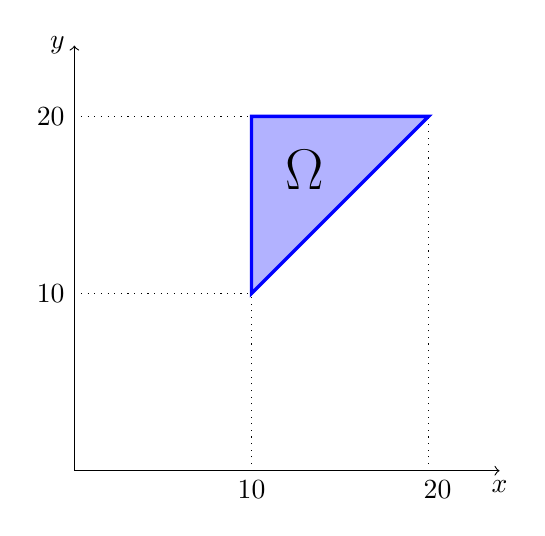
\begin{tikzpicture}[x=0.45cm,y=0.45cm,baseline=(current bounding box.center)]
        \draw[->] (0,0) -- (12,0) node[below] {$x$};
        \draw[->] (0,0) -- (0,12) node[left] {$y$};
        \draw (5,5) -- (10,10) -- (5,10) -- cycle;
        \draw[dotted] (5,0) -- (5,5);
        \draw[dotted] (0,5) -- (5,5);
        \draw[dotted] (10,0) -- (10,10);
        \draw[dotted] (0,10) -- (5,10);
        \node[left] at (0,10) {$20$};
        \node[left] at (0,5) {$10$};
        \node[below] at (10.25,0) {$20$};
        \node[below] at (5,0) {$10$};
        \filldraw[blue, very thick, fill opacity=0.3] (5,5) -- (10,10) -- (5,10) -- cycle;
        \node at (6.5,8.5) {\huge $\Omega$};
    \end{tikzpicture}
    \end{minipage}
    &
    \begin{minipage}{0.45\textwidth}
    \textbf{(a)}\hspace{4pt}
    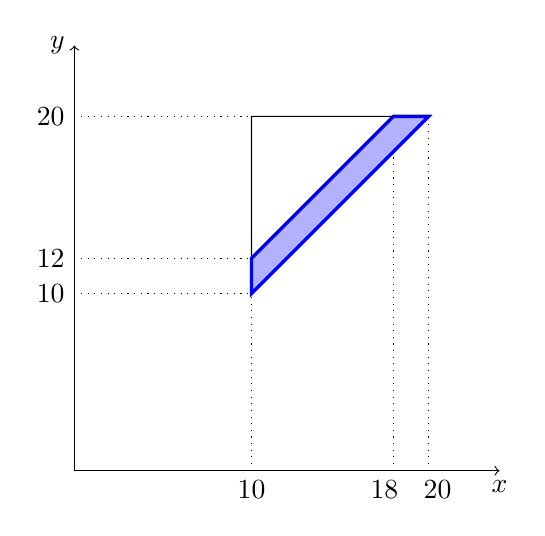
\begin{tikzpicture}[x=0.45cm,y=0.45cm,baseline=(current bounding box.center)]
        \draw[->] (0,0) -- (12,0) node[below] {$x$};
        \draw[->] (0,0) -- (0,12) node[left] {$y$};
        \draw (5,5) -- (10,10) -- (5,10) -- cycle;
        \draw[dotted] (5,0) -- (5,5);
        \draw[dotted] (0,5) -- (5,5);
        \draw[dotted] (10,0) -- (10,10);
        \draw[dotted] (0,10) -- (5,10);
        \node[left] at (0,10) {$20$};
        \node[left] at (0,5) {$10$};
        \node[below] at (10.25,0) {$20$};
        \node[below] at (5,0) {$10$};
        \filldraw[blue, very thick, fill opacity=0.3] (5,5) -- (10,10) -- (9,10) -- (5,6) -- cycle;
        \draw[dotted] (0,6) -- (5,6);
        \draw[dotted] (9,0) -- (9,9);
        \node[left] at (0,6) {$12$};
        \node[below] at (8.75,0) {$18$};
    \end{tikzpicture}
    \end{minipage}
    \\[8mm]
    \begin{minipage}{0.45\textwidth}
    \textbf{(b)}\hspace{4pt}
    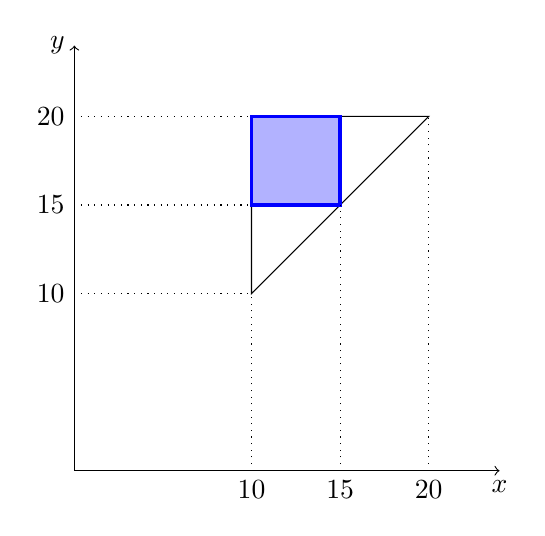
\begin{tikzpicture}[x=0.45cm,y=0.45cm,baseline=(current bounding box.center)]
        \draw[->] (0,0) -- (12,0) node[below] {$x$};
        \draw[->] (0,0) -- (0,12) node[left] {$y$};
        \draw (5,5) -- (10,10) -- (5,10) -- cycle;
        \draw[dotted] (5,0) -- (5,5);
        \draw[dotted] (0,5) -- (5,5);
        \draw[dotted] (10,0) -- (10,10);
        \draw[dotted] (0,10) -- (5,10);
        \node[left] at (0,10) {$20$};
        \node[left] at (0,5) {$10$};
        \node[below] at (10,0) {$20$};
        \node[below] at (5,0) {$10$};
        \filldraw[blue, very thick, fill opacity=0.3] (5,10) -- (7.5,10) -- (7.5,7.5) -- (5,7.5) -- cycle;
        \draw[dotted] (7.5,0) -- (7.5,7.5);
        \draw[dotted] (0,7.5) -- (5,7.5);
        \node[left] at (0,7.5) {$15$};
        \node[below] at (7.5,0) {$15$};
    \end{tikzpicture}
    \end{minipage}
    &
    \begin{minipage}{0.45\textwidth}
    \textbf{(c)}\hspace{4pt}
    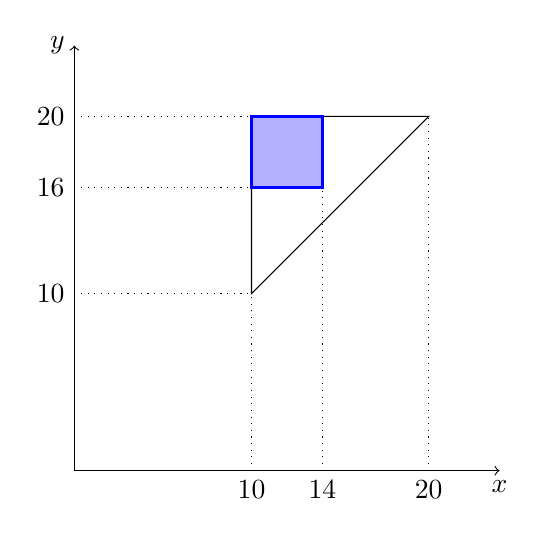
\begin{tikzpicture}[x=0.45cm,y=0.45cm,baseline=(current bounding box.center)]
        \draw[->] (0,0) -- (12,0) node[below] {$x$};
        \draw[->] (0,0) -- (0,12) node[left] {$y$};
        \draw (5,5) -- (10,10) -- (5,10) -- cycle;
        \draw[dotted] (5,0) -- (5,5);
        \draw[dotted] (0,5) -- (5,5);
        \draw[dotted] (10,0) -- (10,10);
        \draw[dotted] (0,10) -- (5,10);
        \node[left] at (0,10) {$20$};
        \node[left] at (0,5) {$10$};
        \node[below] at (10,0) {$20$};
        \node[below] at (5,0) {$10$};
        \filldraw[blue, very thick, fill opacity=0.3] (5,10) -- (7,10) -- (7,8) -- (5,8) -- cycle;
        \draw[dotted] (7,0) -- (7,8);
        \draw[dotted] (0,8) -- (5,8);
        \node[left] at (0,8) {$16$};
        \node[below] at (7,0) {$14$};
    \end{tikzpicture}
    \end{minipage}
    \\[8mm]
    \begin{minipage}{0.45\textwidth}
    \textbf{(d)}\hspace{4pt}
    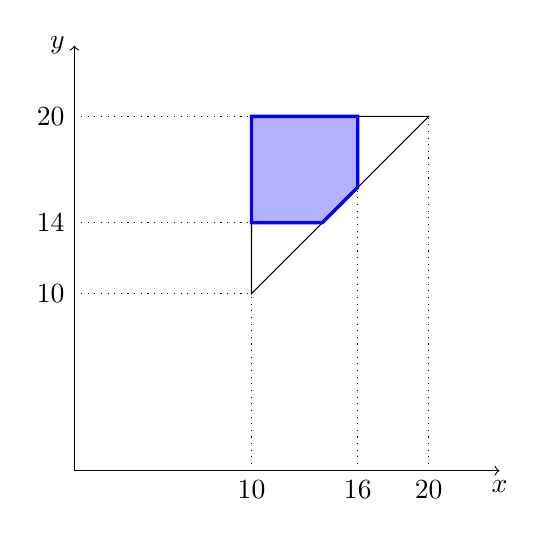
\begin{tikzpicture}[x=0.45cm,y=0.45cm,baseline=(current bounding box.center)]
        \draw[->] (0,0) -- (12,0) node[below] {$x$};
        \draw[->] (0,0) -- (0,12) node[left] {$y$};
        \draw (5,5) -- (10,10) -- (5,10) -- cycle;
        \draw[dotted] (5,0) -- (5,5);
        \draw[dotted] (0,5) -- (5,5);
        \draw[dotted] (10,0) -- (10,10);
        \draw[dotted] (0,10) -- (5,10);
        \node[left] at (0,10) {$20$};
        \node[left] at (0,5) {$10$};
        \node[below] at (10,0) {$20$};
        \node[below] at (5,0) {$10$};
        \filldraw[blue, very thick, fill opacity=0.3] (5,10) -- (8,10) -- (8,8) -- (7,7) -- (5,7) -- cycle;
        \draw[dotted] (8,0) -- (8,8);
        \draw[dotted] (0,7) -- (5,7);
        \node[left] at (0,7) {$14$};
        \node[below] at (8,0) {$16$};
    \end{tikzpicture}
    \end{minipage}
    &
    \begin{minipage}{0.45\textwidth}
    \textbf{(e)}\hspace{4pt}
    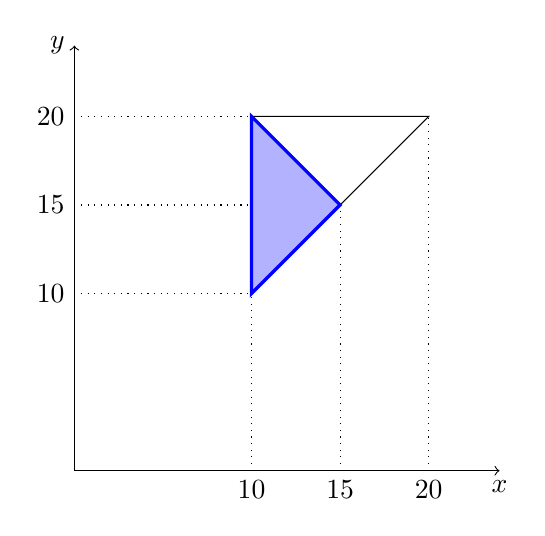
\begin{tikzpicture}[x=0.45cm,y=0.45cm,baseline=(current bounding box.center)]
        \draw[->] (0,0) -- (12,0) node[below] {$x$};
        \draw[->] (0,0) -- (0,12) node[left] {$y$};
        \draw (5,5) -- (10,10) -- (5,10) -- cycle;
        \draw[dotted] (5,0) -- (5,5);
        \draw[dotted] (0,5) -- (5,5);
        \draw[dotted] (10,0) -- (10,10);
        \draw[dotted] (0,10) -- (5,10);
        \node[left] at (0,10) {$20$};
        \node[left] at (0,5) {$10$};
        \node[below] at (10,0) {$20$};
        \node[below] at (5,0) {$10$};
        \filldraw[blue, very thick, fill opacity=0.3] (5,5) -- (7.5,7.5) -- (5,10) -- cycle;
        \draw[dotted] (7.5,0) -- (7.5,7.5);
        \draw[dotted] (0,7.5) -- (5,7.5);
        \node[left] at (0,7.5) {$15$};
        \node[below] at (7.5,0) {$15$};
    \end{tikzpicture}
    \end{minipage}
    \end{tabular}
    \end{center}
    (try to find mathematical justifications for these shapes).
\end{sol}

\begin{sol}{complement-probability}
    We have already established finite additivity in Problem~\ref{prob:finiteadd}, which impllies that
    \[
        \PP(A)+\PP(\overline{A})=\PP(A\cup\overline{A})=\PP(\Omega)=1,
    \]
    hence $\PP(\overline{A})=1-\PP(A)$.
\end{sol}

\begin{sol}{shootingthreetimes}
    \begin{enumerate}
        \item[(a)] $\PP(\text{3 hits}) = \PP(A_1\cap A_2\cap A_3) = P_1P_2P_3$.
        \item[(b)] $\PP(\text{2 hits}) = \PP(A_1\cap A_2\cap\overline{A_3}) + \PP(A_1\cap\overline{A_2}\cap A_3) + \PP(\overline{A_1}\cap A_2\cap A_3) = \\
        \hphantom{\PP(\text{2 hits})} = P_1P_2(1-P_3) + P_1(1-P_2)P_3 + (1-P_1)P_2P_3$.
        \item[(c)] $\PP(\text{at least 2 hits}) = \PP(\text{3 hits}) + \PP(\text{2 hits}) = \\
        \hphantom{\PP(\text{at least 2 hits})} = P_1P_2P_3 + P_1P_2(1-P_3) + P_1(1-P_2)P_3 + (1-P_1)P_2P_3$.
        \item[(d)] $\PP(\text{0 hits}) = \PP(\overline{A_1}\cap\overline{A_2}\cap\overline{A_3})=(1-P_1)(1-P_2)(1-P_3)$.
        \item[(e)] $\PP(\text{at lease 1 hit})=1-\PP(\text{0 hits})=1-(1-P_1)(1-P_2)(1-P_3)$.
        \item[(f)] $\PP(\text{even hits})=\PP(\text{0 hits})+\PP(\text{2 hits})=\\
        \hphantom{\PP(\text{even hits})}=(1-P_1)(1-P_2)(1-P_3)+P_1P_2(1-P_3) + P_1(1-P_2)P_3 + (1-P_1)P_2P_3$.
        \item[(g)] $\PP(\text{odd hits})=\PP(\text{1 hit})+\PP(\text{3 hits})=\\
        \hphantom{\PP(\text{odd hits})}=P_1(1-P_2)(1-P_3)+(1-P_1)P_2(1-P_3)+(1-P_1)(1-P_2)P_3+P_1P_2P_3$.
    \end{enumerate}
\end{sol}